\chapter{Metodologia}
\label{metodologia}

O Software Livre possui um mecanismo de produção colaborativo e dinâmico 
e possui uma organização composta por um conjunto de pessoas que usa e desenvolve 
um único software livre, contribuindo para uma base comum de código-fonte e 
conhecimento~\cite{reis2003caracterizacc}.

O sucesso de um projeto de código aberto depende fortemente da participação de 
voluntária de um grande número de desenvolvedores. É necessário que os novos 
desenvolvedores se sintam motivados e engajados para que eles continuem no 
projeto\\~\cite{qureshi2010socialization}.

Desta forma, a entrada de membros nas comunidades se torna uma das atividades que
merece atenção. Grande parte dos desenvolvedores desistem de contribuir com o 
projeto nas primeiras interações com a comunidade e com o projeto sem chegar,
ao menos, à levantar o ambiente do software.

Com projetos de software público não é diferente, apesar de haver um portal que
centraliza as informações do projeto, queremos averiguar se as barreiras levantadas
para projetos de software livre, mostradas no Capítulo~\ref{barreirasSL}, se aplicam
a projetos de software público e se além dessas barreiras já mapeadas, existem outras 
barreiras específicas, devido as características desses projetos.

O modelo típico do software livre se diferencia em muitos aspectos 
com a forma que o governo brasileiro desenvolve software, onde se estabelece um 
rígido processo, portanto essa pesquisa visa entender se existem mais barreiras 
para se desenvolver um projeto de software público do que as já mapeadas para 
desenvolver software livre.



\section{Questão de pesquisa}

As boas práticas de desenvolvimento a serem utilizadas em um projeto de software 
dependem do contexto, uma equipe que desenvolve software livre utiliza
meios diferentes para gerenciar o próprio projeto, que pode conter especificidades 
que impedem o uso de determinadas práticas impostas pelo governo federal para controle
do desenvolvimento de software. 

Dessa forma, com base no problema proposto, elaboramos a seguinte questão:

\begin{itemize}
\item \emph{QP1:Existem mais barreiras para começar a contribuir 
com um projeto de software público do que com um projeto de software livre?}

\end{itemize}

Acreditamos que a forma com que o governo brasileiro adota os software públicos
e trabalha no desenvolvimento pode gerar mais barreiras no desenvolvimento que 
não se aplicam ou não estão presentes no desenvolvimento de software livre. O
Governo Federal possui uma estrutura rígida de cargos, onde se estabelece um
distanciamento daqueles que demandam produtos de software daqueles que desenvolvem
software e procuramos saber se esta forma não causa ainda mais dificuldades no 
desenvolvimento.

\section{Pesquisa com as comunidades}

Nós reproduzimos a pesquisa elencada no trabalho de \citeonline{steinmancher2015} 
da maneira que foi apresentada no Capítulo \ref{barreirasSL}, no ambiente
do SPB com algumas adaptações para a realidade e o tempo do trabalho de conclusão
de curso.

Para identificar as barreiras para contribuir com software livre, \citeonline{steinmancher2015} conduziu a 
pesquisa qualitativa com base em um estudo sistemático da bibliografia existente no
assunto, relato de estudantes que contribuiram com software livre, questinário com 
questões abertas aplicado a desenvolvedores de software livre e entrevistas com 
desenvolvedores com diferentes níveis de formação e experiência em desenvolvimento
de software livre.
 
Com o objetivo de levantar as barreiras para contribuir com software público, adaptamos
a pesquisa do Igor, primeiramente utilizando como revisão sistemática a pesquisa feita 
pelo Igor das barreiras para software livre, traduzimos e adaptamos os questinários
por ele produzido para que atendesse a realidade do software público, como pode ser 
visto nos Anexos~\ref{anexo b}, \ref{anexo c} e \ref{anexo e}. Para o contexto do 
trabalho de conclusão de curso julgamos que com as barreiras levantadas por estes 
questionários já seriam suficientes, dessa forma optamos por não fazer as entrevistas.

Nós utilizamos as 6 comunidades que acreditávamos ser mais ativas
no Portal do Software Público com base nas participações dos membros nas listas de 
discussão das comunidades e importância estratégica dentro do governo, são elas:

\begin{itemize}

\item Noosfero.gov\footnote{https://softwarepublico.gov.br/social/noosferogov}: 
O noosfero é uma plataforma web para contrução de redes sociais. Está dentro do
SPB como um software livre para a utilização do SERPRO\footnote{http://www.serpro.gov.br/}, 

\item CACIC\footnote{https://softwarepublico.gov.br/social/cacic}: Foi o primeiro 
software público do SPB, é um sistema baseado em agentes que é capaz de obter um 
diagnóstico preciso do parque computacional e fornecer informações de diversos tipos 
de dispositivos e softwares presentes em um computador.

\item SAE - Sistema de apoio educacional\footnote{https://softwarepublico.gov.br/social/sae}:
É um projeto antigo dentro do SPB, utilizado em processos educacionais personalizados no 
ensino presencial e a distância.  

\item I-Educar\footnote{https://softwarepublico.gov.br/social/i-educar}: Software público de 
gestão escolar utilizado por diversos estados, incluindo o Distrito Federal. Está presente
no SPB desde a versão antiga do portal.

\item E-SIC\footnote{https://softwarepublico.gov.br/social/e-sic-livre}: É uma solução voltada 
para a gestão de atendimento ao público baseado em perguntas e respostas, e visa 
oferecer aos municípios um serviço de pleno acordo com a Lei de Acesso à Informação (LAI).
Um projeto novo, foi lançado já na versão nova do SPB, não passando assim pelos 
probelmas enfrentados pelas comunidades na versão antiga do SPB.

\item SEI - Sistema Eletrônico de informações\footnote{https://softwarepublico.gov.br/social/sei}:
É uma plataforma que engloba um conjunto de módulos e funcionalidades que promovem 
a eficiência administrativa. Não é classificado como software público mas foi contruído com
recursos públicos e utiliza hoje a infraestrutura do SPB para sua manutenção.

\end{itemize}


Nós enviamos a estas comunidades a mensagem presente no anexo \ref{anexo a}
com o pedido que participassem da pesquisa mostrando o objetivo da mesma. Nosso objetivo 
era atingir àqueles que contribuem com os projetos. Deixamos o questionário disponível 
para que fosse respondido por 2 meses, enviando a mensagem apresentda em duas ocasiões.

Nós procuramos uma comunidade na qual os desenvolvedores tivessem desistido
de desenvolver o software, pedimos ajuda aos mantenedores do SPB no MPOG e eles nos 
indicaram o projeto OASIS\footnote{https://softwarepublico.gov.br/social/oasis} que 
está ativo no SPB desde o antigo portal mas que a algum tempo não havia alterações
na comunidade, e então enviamos um questionáo específico, como consta no Anexo~\ref{anexo c} 
para desenvolvedores que desistiram de contribuir, mas não obtivemos nenhuma resposta. 

Para completar a pesquisa, enviamos outro questionários para alguns dos gestores dos
projetos escolhidos, que são chamados no SPB de coordenadores das comunidades e 
são membros mais experientes no projeto por meio da mensagem apresentada no Anexo~\ref{anexo d}, 
para que obtivéssemos também a visão deles em relação a entrada de novos contribuidores aos projetos. 

Para a análise dos dados coletados com os questionários, utilizamos \textit{Ground Theory}, 
explicada anteriormente no capítulo~\ref{barreirasSL}.

Antes da pesquisa com as comunidades nós iniciamos o desenvolvimento do novo portal
FlossCoach criando um protótipo inicial com o cadastro dos projetos e de usuários 
conforme o portal atual o que será explicado em detalhes a seguir. 

\section{Metodologia de desenvolvimento}

O desenvolvimento do portal FlossCoach foi dividido em 3 fases, com a intenção de 
automatizar o FlossCoach iniciamos o desenvolvimento com um protótipo funcional, no qual 
um usuário poderia fazer diretamente o cadastro de seu projeto após fazer um cadastro de 
usuário. Realizamos uma reengenharia do portal observando quais as funcionalidades 
que o portal já possui e reimplementamos em \textit{ruby on rails} e \textit{bootstrap}.

Após esta primeira etapa, O Igor Steinmancher montou uma equipe de desenvolvimento 
para melhorar o \textit{front end} do projeto e implementar outras funcionalidades, 
esta equipe esta alocada na USP, juntamente com o Igor. Nesse período em que o Igor 
estava tomando conhecimento do código por nós desenvolvido e montando a equipe para
ajudar com o desenvolvimento na USP, nós traduzimos, adaptamos e aplicamos os questionários
às comunidades escolhidas de projetos de software público.

Para usar os questinários do trabalho de \citeonline{steinmancher2015} nós tivemos que traduzi-los pois se tratando de
software público e de projetos que estão ligados ao governo, os próprios membros 
do governo não aceitariam responder o questionário em inglês. Onde havia software 
livre, substituímos por software público por exemplo, na questão sobre motivação
do questionário para desenvolvedores, presente no Anexo~\ref{anexo b}, a questão 
tirada do questionário do Igor, ``\textit{What motivated you to start contributing 
to an OSS project?}'', em nosso questionário passou a ser ``Qual a sua motivação para 
contribuir com software público?''.

Com o projeto já em uma fase mais madura do desenvolvimento, o professor orientador
deste trabalho, Paulo Meirelles, ministra uma disciplina de Manutenção e Evolução de
Software, na qual os alunos tem que dar manutenção em um software livre e o FlossCoach
passou a ser um dos projetos desta disciplinas. Um grupo ficou responsável por dar 
manutenções corretivas e evolutivas no projeto.

As manutenções a serem implementadas pelos alunos foram previamente discutidas
por nós em conjunto com a equipe na USP e ao menos uma vez por semana eu estive junto com a 
equipe de alunos da disciplina para dar orientações, tirar dúvidas do projeto
e desenvolver em parceria, além de revisar o código elaborado pelas equipes.
 
A disciplina utiliza as práticas aplicadas às metodologias ágeis, dividimos o tempo 
da disciplina em \textit{sprints} de duas semanas nas quais no início de cada uma 
fazíamos uma reunião com toda a equipe para decidir quais \textit{issues} iríamos 
desenvolver naquele período. Utilizamos a prática de programação em pares, alternando
os pares ao final das \textit{sprints} para circular o conhecimento dentro da equipe.
Fazíamos \textit{stand up}, reuniões de 15 minutos, em pé para que cada dupla compartilhasse
o andamento de suas tarefas e tirasse eventuais dúvidas com a equipe e ao final da sprint 
fazíamos uma reunião de revisão da \textit{sprint} para verificar quais \textit{issues} foram finalizadas e quais 
necessitam de mais tempo e serão passadas para a próxima \textit{sprint} como ilustrado na Figura~\ref{fig:disciplina}.

\begin{figure}[h]
	\centering
		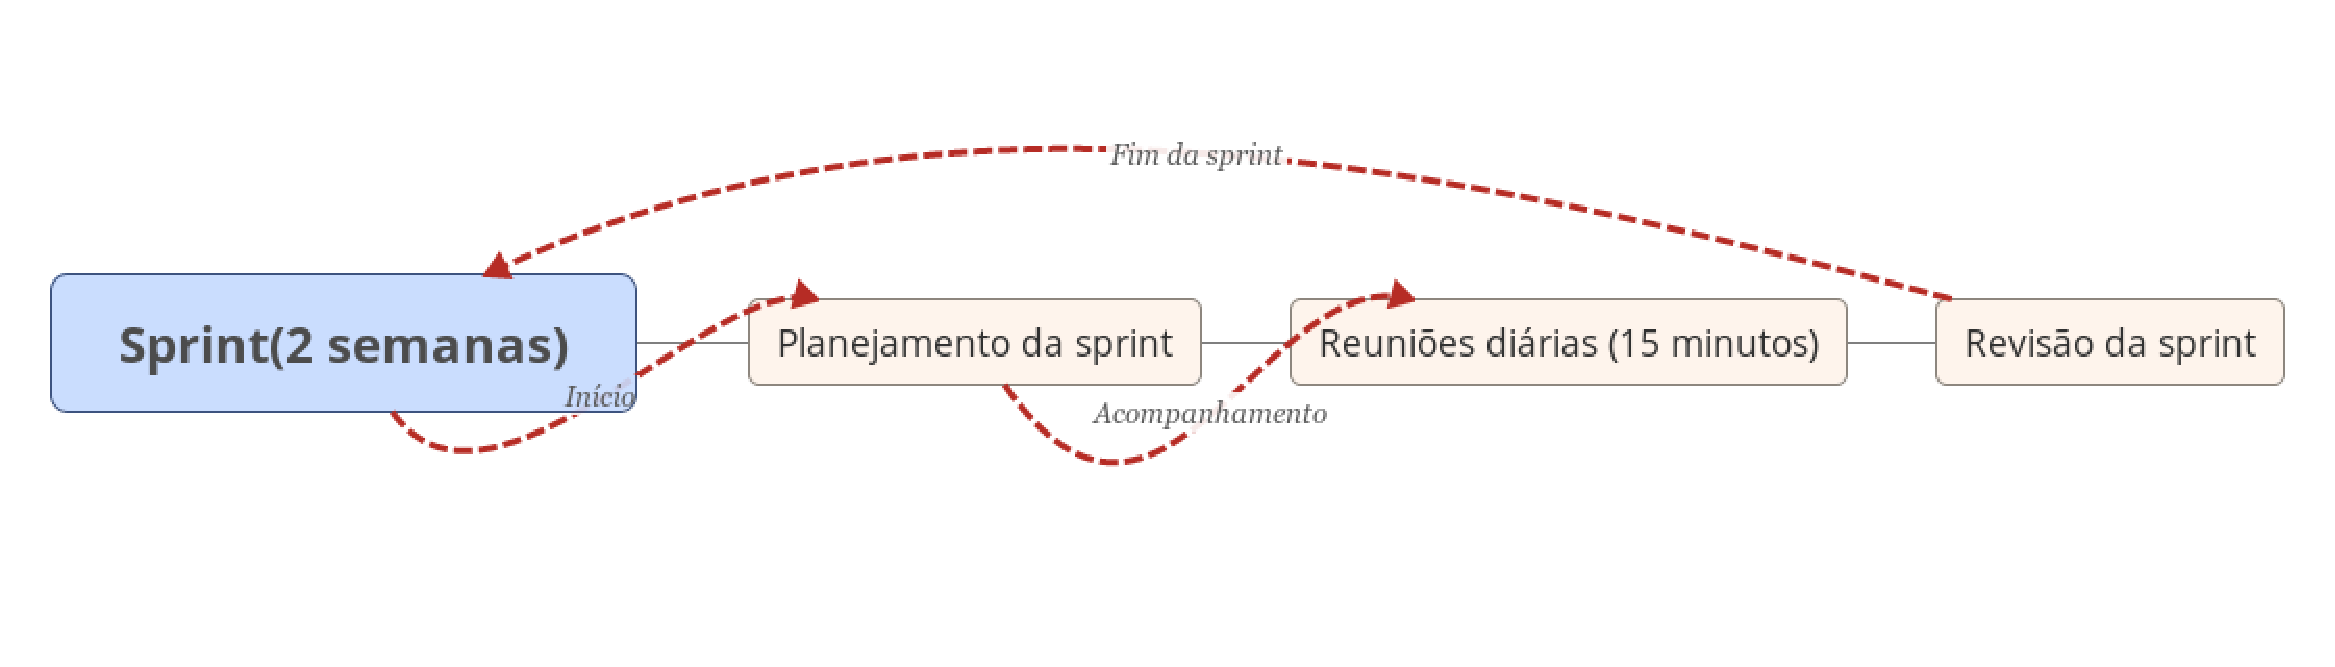
\includegraphics[keepaspectratio=true,scale=0.4]{figuras/Sprint.eps}
	\caption{Dinâmica do desenvolvimento na disciplina Manutenção e Evolução de Software.}
	\label{fig:disciplina}
\end{figure}

Meus papéis no desenvolvimento do projeto foram diferentes nas 3 fases do projeto, na 
primeira fase trabalhei como desenvolvedora do projeto iniciando o protótipo funcional
do FlossCoach, na segunda fase trabalhei como arquiteta de software ajudando a tomar as
decisões arquiteturais do projeto em conjunto com a equipe na USP e, na terceira fase,
continuei meu trabalho de arquiteta contribuindo nas decisões do projeto além de ser
revisora dos códigos feitos pelos alunos da disciplina além de voltar a trabalhar no
desenvolvimento para ajudar os alunos nas tarefas mais complicadas. Na disciplina 
acumulei também o papel de cliente e dessa forma passava para os alunos da disciplina
as decisões feitas pela equipe na USP e os próximos passos do desenvolvimento. 


